% !TeX spellcheck = pt_BR

\chapter{A área abaixo do gráfico $v$ por $t.$} \label{apendice_areagraficovxt}



A ideia de se calcular a área abaixo de certos gráficos aparecerá ao longo deste livro em três contextos distintos: ao calcular a distância percorrida por um corpo de velocidade variável; ao calcular o impulso de uma força que muda com o tempo; e ao computar o trabalho realizado por uma força que varia com a posição. Vejamos como o conceito da área é relevante nesses contextos.


\section*{Equações que exigem constância}

Considere a primeira definição que fizemos de velocidade escalar média: $v = d/\Delta t.$ Para um corpo que se move com velocidade \textit{constante} $v$ durante um intervalo de tempo $\Delta t$, a distância percorrida é simplesmente

$$ d = v \cdot \Delta t. $$

No gráfico de $v$ por $t$, a velocidade constante corresponde a uma linha horizontal. A distância $d = v \cdot \Delta t$ é a área do retângulo de altura $v$ e largura $\Delta t$ abaixo dessa linha, como ilustra a Figura~\ref{fig_apendice_area_constante}.



\vspace{0.3cm}
{
\centering
\begin{tikzpicture}
  \begin{scope}[blend mode=multiply]
    \node {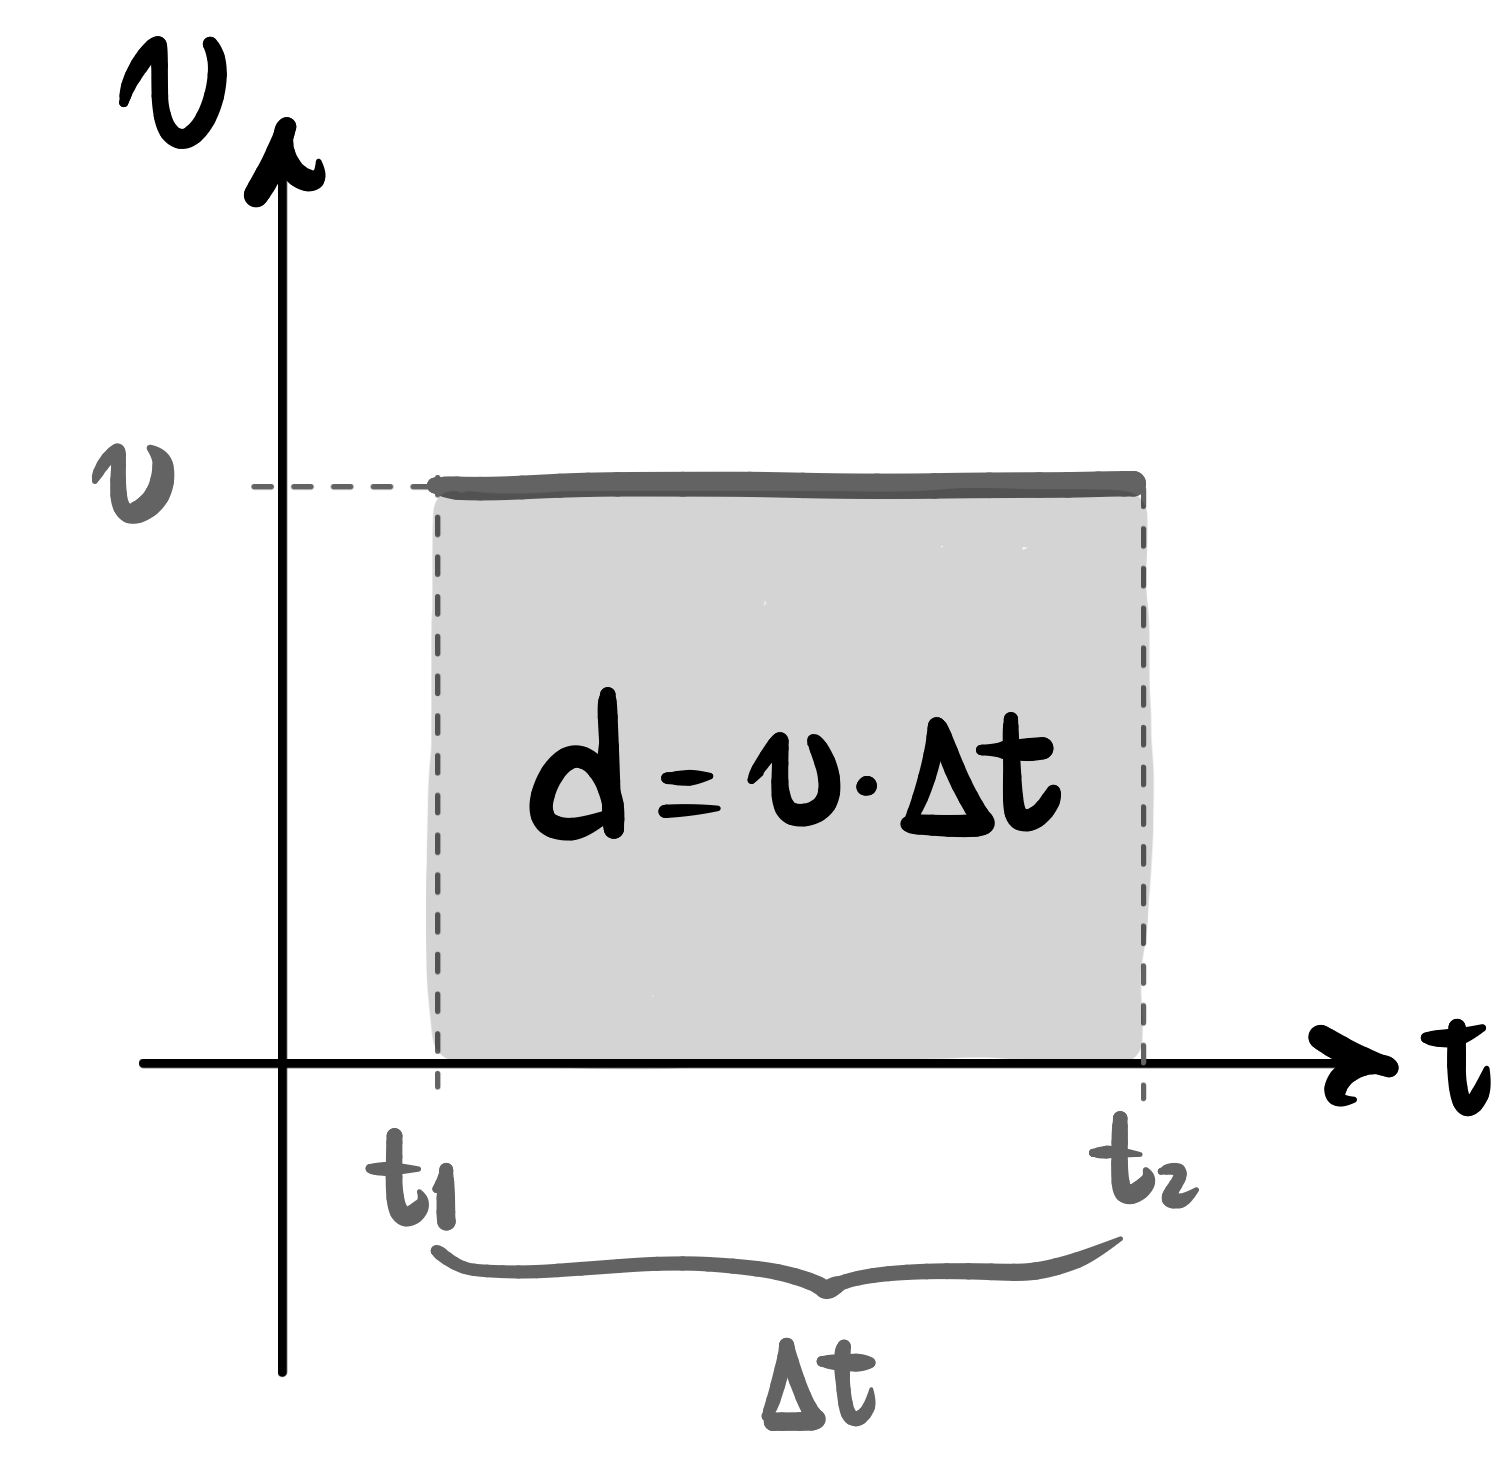
\includegraphics[width=0.35\linewidth]{imagensapendices/areagrafico01.png}};
  \end{scope}
\end{tikzpicture}
\captionof{figure}{Velocidade constante: a distância é exatamente a área do retângulo.}
\label{fig_apendice_area_constante}
} 
\vspace{0.3cm}





Até aqui, tudo simples. O problema começa quando a velocidade não é constante. Na vida real, os corpos raramente se movem com velocidade constante. Um carro que acelera, uma bola que cai, um atleta correndo --- em todos esses casos, $v$ muda a cada instante. Nessa situação, a equação $d = v \cdot \Delta t$ não faz mais sentido diretamente: qual valor de $v$ usaríamos? O do início? O do fim? A média? Nenhum desses é exato: precisamos de outro caminho.


A solução é analisar o movimento fatiando o tempo. A ideia central é esta: mesmo que a velocidade varie durante um certo intervalo de tempo longo, em um intervalo de tempo \textit{muito pequeno} $\Delta t_i$ ela mal muda --- é como se fosse constante naquele instante. E se for aproximadamente constante, podemos usar $d \approx v \cdot \Delta t$:

$$ \Delta d_i \approx v_i \cdot \Delta t_i. $$

Ou seja, naquele intervalo de tempo $\Delta t_i$ muito pequeno --- que é um subintervalo dentro do intervalo de tempo maior $\Delta t$ ao longo do qual o corpo se move ---, o intervalo é mesmo tão pequeno que a velocidade quase não muda, de modo que a distância percorrida $\Delta d_i$ pode ser computada pela relação acima.

Contudo, note que, geometricamente, $v_i \cdot \Delta t_i$ é a área de um retângulo fino: altura $v_i$, largura $\Delta t_i$, como mostra a primeira imagem da Figura~\ref{fig_apendice_area_fatias}.


\vspace{0.3cm}
{
\centering
\begin{tikzpicture}
  \begin{scope}[blend mode=multiply]
    \node {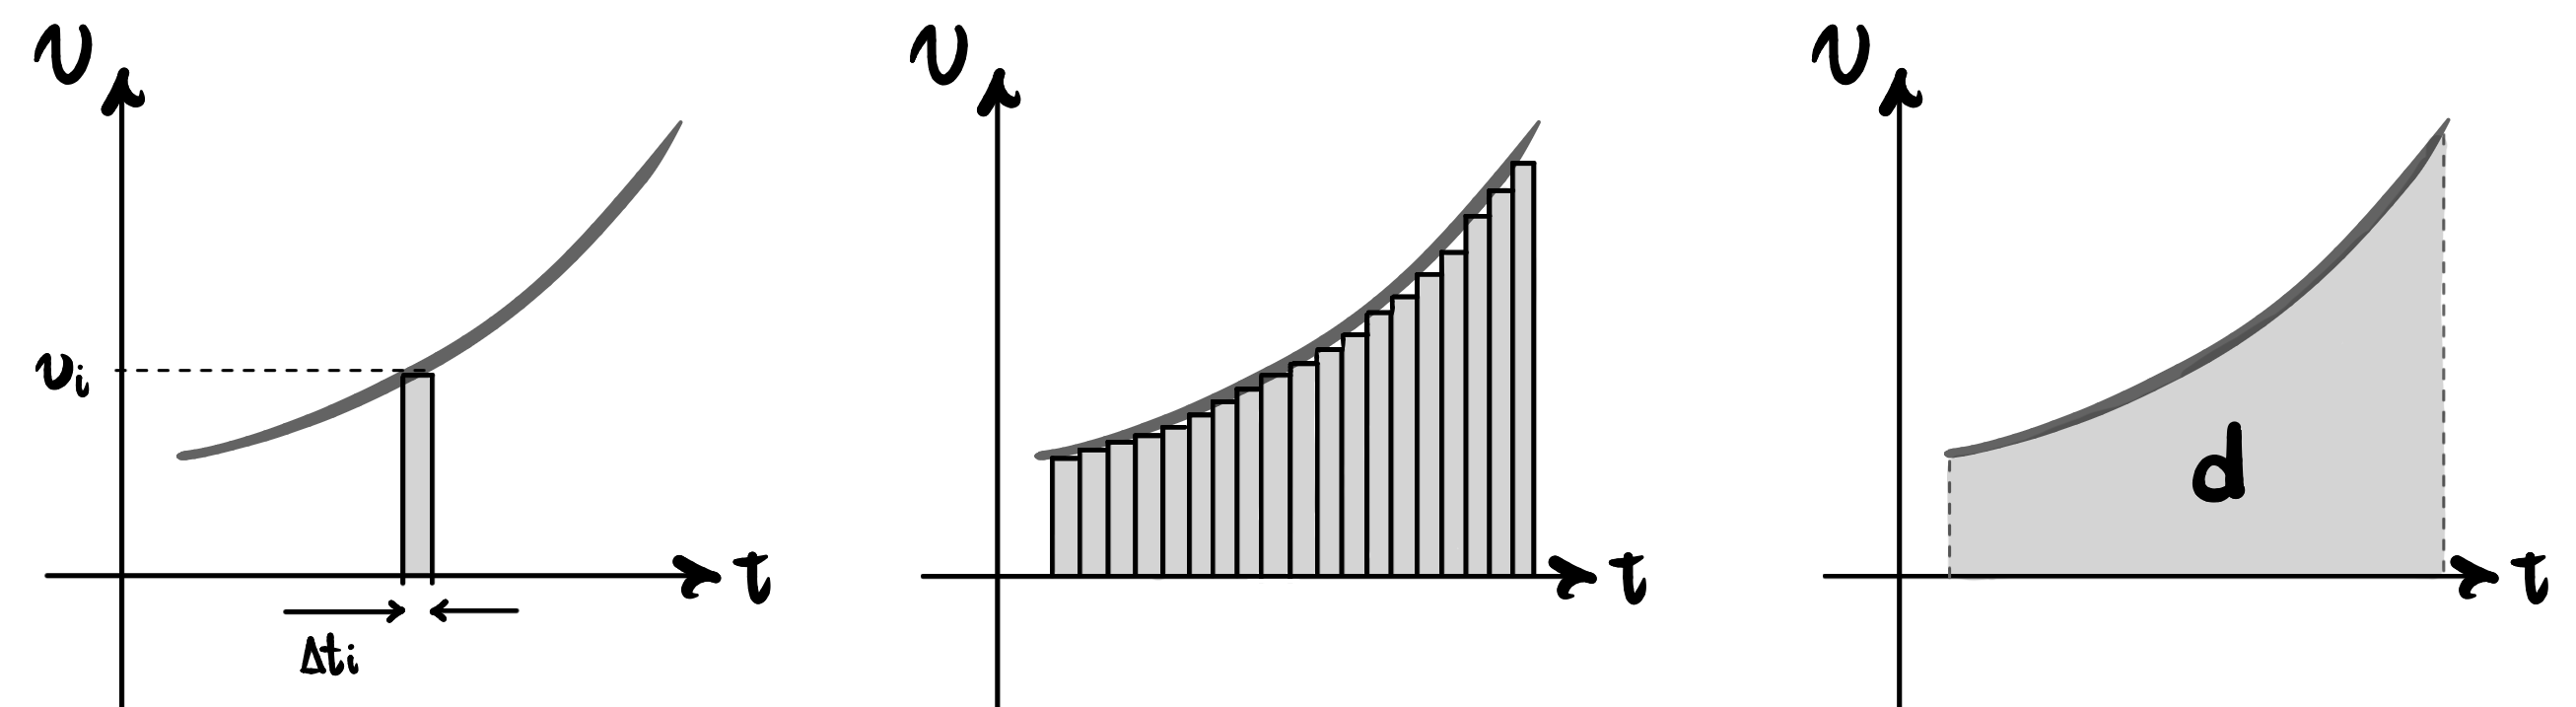
\includegraphics[width=0.95\linewidth]{imagensapendices/areagrafico02.png}};
  \end{scope}
\end{tikzpicture}
\captionof{figure}{Da esquerda para a direita: uma fatia isolada com altura $v_i$ e largura $\Delta t_i$; a soma de todas as fatias (aproximação da área); no limite de fatias infinitamente finas, a área exata corresponde à distância total percorrida.}
\label{fig_apendice_area_fatias}
} 
\vspace{0.3cm}


Assim, se para o intervalo de tempo bem curto $\Delta t_i$ a distância percorrida seria a área do retângulo da primeira imagem da Figura \ref{fig_apendice_area_fatias}, podemos dividir o intervalo de tempo total de movimento $\Delta t$ em vários intervalos $\Delta t_i$ muito pequenos, de modo que, nestes intervalos, a velocidade praticamente não mude e seja possível aplicar $\Delta d_i = v_i \Delta t_i.$ Isso é o que aparece na segunda imagem da figura.

Assim, se os intervalos todos forem suficientemente pequenos, a soma das áreas dos retângulos fornecerá a área abaixo do gráfico, como mostra a terceira imagem da figura. Isto é, a distância total percorrida é a soma das contribuições de todas as fatias:

$$ d \;=\; \sum_i \Delta d_i \;\approx\; \sum_i v_i \cdot \Delta t_i. $$

Cada termo $v_i \cdot \Delta t_i$ é a área de um retângulo fino. A soma de todos eles preenche, de forma aproximada, a região entre a curva e o eixo do tempo. Quanto mais finas as fatias --- quanto menor cada $\Delta t_i$ --- menor o erro cometido ao tratar $v$ como constante em cada uma. No limite em que as fatias se tornam infinitamente finas, a aproximação se torna exata:

$$  d \;=\; \text{área sob a curva } v(t). $$

\begin{quote}
A distância percorrida por um corpo --- mesmo que sua velocidade varie
arbitrariamente --- é sempre igual à área da região delimitada pelo gráfico
$v(t)$, pelo eixo do tempo e pelas verticais nos instantes inicial e final.
\end{quote}

O ponto fundamental que vale destacar: a equação $d = v \cdot \Delta t$ só era válida para velocidade constante. O argumento das fatias não criou uma equação nova --- ele estendeu a validade da equação original a um domínio mais amplo, ao transformar \textit{``constante''} em \textit{``localmente constante em cada fatia infinitesimal''}. É assim que a Física expande seus instrumentos sem precisar reescrevê-los do zero.

Uma pergunta interessante seria:

\begin{center}
    \textit{O argumento vale quando a grandeza é negativa?}
\end{center}



Sim --- com uma ressalva. Se $v < 0$ em algum trecho (o corpo se move no sentido negativo), os retângulos nesse trecho têm altura negativa, e sua área contribui negativamente para a soma. O resultado é o \textit{deslocamento} --- que pode ser menor do que a distância total percorrida. A área \textit{algébrica} sob a curva fornece o deslocamento; a soma dos módulos das áreas em cada trecho fornece a distância total percorrida.


\section*{O mesmo argumento em diferentes contextos}

A lógica desenvolvida acima não depende de nenhuma propriedade especial da velocidade. O argumento é geral: sempre que tivermos uma equação $Y = X \cdot Z$ válida para $X$ constante, a área sob o gráfico de $X$ em função de $Z$ fornece o valor de $Y$ mesmo quando $X$ varia.

\textbf{Força $\times$ Tempo $\rightarrow$ Impulso.} A equação $I = F \cdot \Delta t$ é estritamente válida apenas para força constante. Quando $F$ varia com o tempo, o mesmo argumento das fatias se aplica: em cada fatia $\Delta t_i$, a força é aproximadamente constante e contribui com $F_i \cdot \Delta t_i$ para o impulso total. A soma de todas as contribuições é a área sob o gráfico $F(t)$.

\textbf{Força $\times$ Deslocamento $\rightarrow$ Trabalho.} A equação $W = F \cdot d$ vale para força constante paralela ao deslocamento. Quando $F$ varia com a posição --- como na força elástica $F = kx$ --- o fatiamento se aplica ao longo do deslocamento. A área sob o gráfico $F(x)$ fornece o trabalho total. 


\vspace{0.3cm}
{
\centering
\begin{tikzpicture}
  \begin{scope}[blend mode=multiply]
    \node {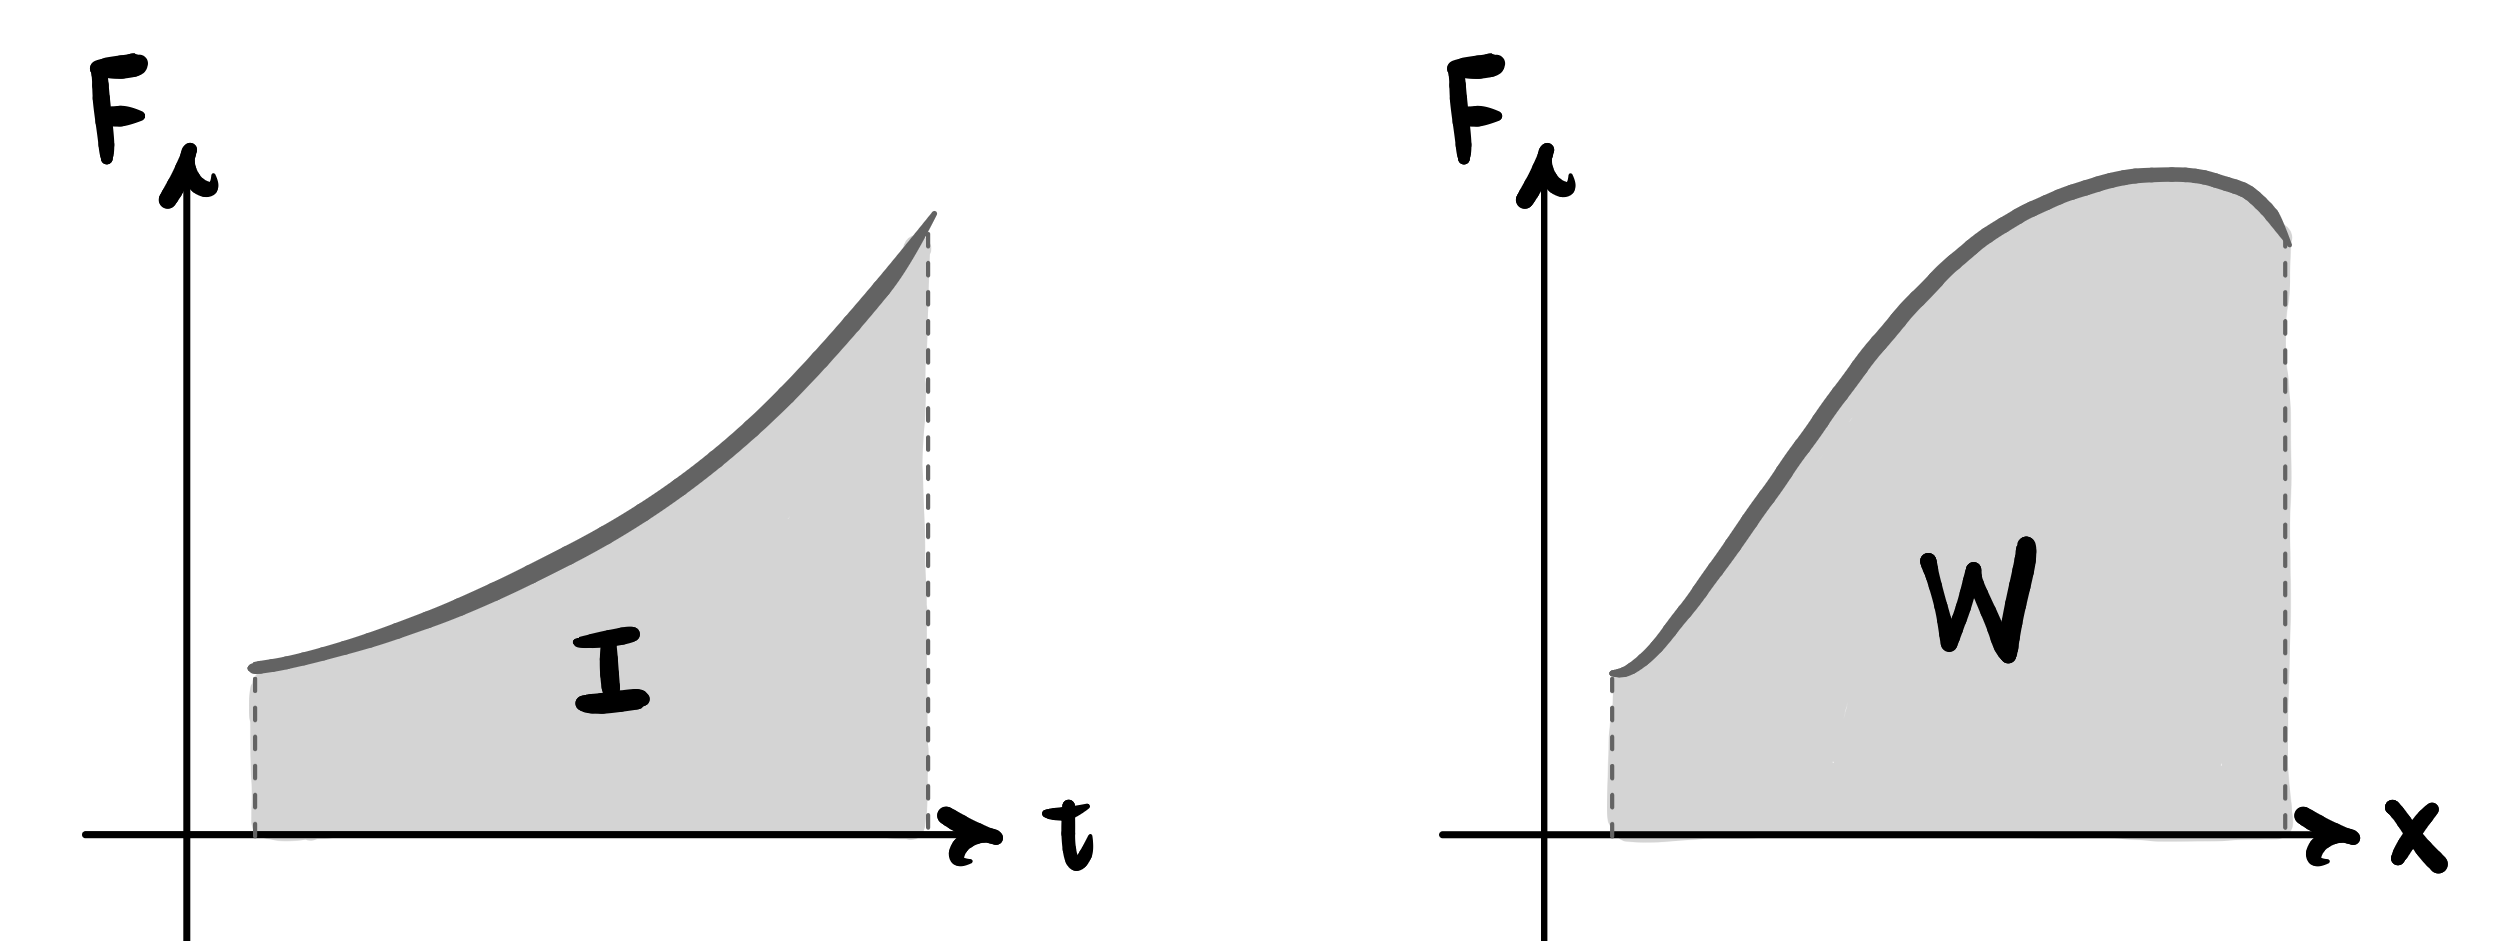
\includegraphics[width=0.75\linewidth]{imagensapendices/areagrafico03.png}};
  \end{scope}
\end{tikzpicture}
\captionof{figure}{O mesmo argumento aplicado a outros gráficos: a área sob $F(t)$ é o impulso; a área sob $F(x)$ é o trabalho.}
\label{fig_apendice_area_aplicacoes}
} 
\vspace{0.3cm}


Nos três casos --- $v(t)$, $F(t)$, $F(x)$ --- o mesmo argumento fornece o mesmo resultado: a área sob o gráfico é o produto acumulado das duas grandezas envolvidas, mesmo quando uma delas varie. A área é a linguagem da variação.